% ============================================================
\chapter{Manipulation de Donn\'ees avec Pandas}
\label{ch:pandas}
% ============================================================

\section{Introduction \`a Pandas}

\textbf{Pandas}\index{Pandas} est la biblioth\`eque centrale de la data science en Python. Elle fournit deux structures de donn\'ees fondamentales : le \py{Series} (vecteur index\'e) et le \py{DataFrame} (tableau index\'e).

\begin{definition}[DataFrame]
Un \textbf{DataFrame} est un tableau bidimensionnel avec des \'etiquettes pour les lignes (index) et les colonnes. Chaque colonne est une \py{Series} de m\^eme longueur.
\end{definition}

\section{Cr\'eation de DataFrames}

\begin{codeblock}[title=\textbf{Python --- Cr\'eation}]
\begin{minted}{python}
import pandas as pd
import numpy as np

# À partir d'un dictionnaire
data = {
    'Nom': ['Alice', 'Bob', 'Charlie', 'Diana'],
    'Âge': [25, 30, 35, 28],
    'Salaire': [45000, 55000, 70000, 52000],
    'Ville': ['Paris', 'Lyon', 'Paris', 'Marseille']
}
df = pd.DataFrame(data)
print(df)
print(f"\nShape : {df.shape}")
print(f"Types :\n{df.dtypes}")
\end{minted}
\end{codeblock}

\begin{codeoutput}
\begin{verbatim}
       Nom  Âge  Salaire      Ville
0    Alice   25    45000      Paris
1      Bob   30    55000       Lyon
2  Charlie   35    70000      Paris
3    Diana   28    52000  Marseille

Shape : (4, 4)
Types :
Nom        object
Âge         int64
Salaire     int64
Ville      object
dtype: object
\end{verbatim}
\end{codeoutput}

\section{Chargement de donn\'ees}

\begin{codeblock}[title=\textbf{Python --- Lecture de fichiers}]
\begin{minted}{python}
# CSV (le plus courant)
# df = pd.read_csv('donnees.csv')
# df = pd.read_csv('donnees.csv', sep=';', encoding='utf-8')

# Depuis Seaborn (jeux de données intégrés)
tips = sns.load_dataset('tips')   # pourboires au restaurant
print(f"Dimensions : {tips.shape}")
print(tips.head(3))
\end{minted}
\end{codeblock}

\begin{codeoutput}
\begin{verbatim}
Dimensions : (244, 7)
   total_bill   tip     sex smoker  day    time  size
0       16.99  1.01  Female     No  Sun  Dinner     2
1       10.34  1.66    Male     No  Sun  Dinner     3
2       21.01  3.50    Male     No  Sun  Dinner     3
\end{verbatim}
\end{codeoutput}

\section{S\'election et indexation}

\begin{formules}[title=\textbf{M\'ethodes de s\'election}]
\begin{tabular}{ll}
\toprule
\textbf{Syntaxe} & \textbf{Description} \\
\midrule
\py{df['col']} & S\'electionner une colonne (Series) \\
\py{df[['c1','c2']]} & S\'electionner plusieurs colonnes \\
\py{df.loc[i, 'col']} & S\'election par \'etiquette \\
\py{df.iloc[i, j]} & S\'election par position \\
\py{df[df['col'] > x]} & Filtrage bool\'een \\
\bottomrule
\end{tabular}
\end{formules}

\begin{codeblock}[title=\textbf{Python --- S\'election}]
\begin{minted}{python}
import seaborn as sns
tips = sns.load_dataset('tips')

# Sélection de colonnes
print("--- Colonne unique ---")
print(tips['total_bill'].head(3))

# Filtrage
gros_pourboires = tips[tips['tip'] > 5]
print(f"\n--- Pourboires > 5$ : {len(gros_pourboires)} lignes ---")
print(gros_pourboires.head(3))

# Sélection combinée
print("\n--- loc : femmes, dimanche ---")
mask = (tips['sex'] == 'Female') & (tips['day'] == 'Sun')
print(tips.loc[mask, ['total_bill', 'tip']].head(3))
\end{minted}
\end{codeblock}

\begin{codeoutput}
\begin{verbatim}
--- Colonne unique ---
0    16.99
1    10.34
2    21.01
Name: total_bill, dtype: float64

--- Pourboires > 5$ : 17 lignes ---
     total_bill   tip   sex smoker  day    time  size
23        39.42  7.58  Male     No  Sat  Dinner     4
44        30.40  5.60  Male     No  Sun  Dinner     4
47        32.40  6.00  Male     No  Sun  Dinner     4

--- loc : femmes, dimanche ---
     total_bill   tip
0         16.99  1.01
5         25.29  4.71
15        21.58  3.92
\end{verbatim}
\end{codeoutput}

\section{Modification et ajout de colonnes}

\begin{codeblock}[title=\textbf{Python --- Nouvelles colonnes}]
\begin{minted}{python}
# Ajouter une colonne calculée
tips['tip_pct'] = (tips['tip'] / tips['total_bill'] * 100).round(1)
print(tips[['total_bill', 'tip', 'tip_pct']].head(5))

# Appliquer une fonction
tips['bill_category'] = tips['total_bill'].apply(
    lambda x: 'Élevé' if x > 30 else ('Moyen' if x > 15 else 'Bas'))
print(tips['bill_category'].value_counts())
\end{minted}
\end{codeblock}

\begin{codeoutput}
\begin{verbatim}
   total_bill   tip  tip_pct
0       16.99  1.01      5.9
1       10.34  1.66     16.1
2       21.01  3.50     16.7
3       23.68  3.31     14.0
4       24.59  3.61     14.7

bill_category
Moyen     111
Bas        69
Élevé      64
Name: count, dtype: int64
\end{verbatim}
\end{codeoutput}

\section{Agr\'egation avec \texttt{groupby}}

\begin{definition}[Split-Apply-Combine]\index{groupby}
Le paradigme \textbf{split-apply-combine} consiste \`a :
\begin{enumerate}
\item \textbf{Split} : diviser les donn\'ees en groupes.
\item \textbf{Apply} : appliquer une fonction (somme, moyenne, comptage\ldots) \`a chaque groupe.
\item \textbf{Combine} : combiner les r\'esultats.
\end{enumerate}
\end{definition}

\begin{center}
\begin{tikzpicture}[
  block/.style={rectangle, draw, fill=#1!15, rounded corners,
    minimum width=2.2cm, minimum height=0.8cm, align=center, font=\small},
  arr/.style={-{Stealth}, thick}
]
\node[block=blue] (data) at (0,0) {Donn\'ees};
\node[block=red] (g1) at (4,1) {Groupe A};
\node[block=red] (g2) at (4,0) {Groupe B};
\node[block=red] (g3) at (4,-1) {Groupe C};
\node[block=green] (r1) at (8,1) {R\'esultat A};
\node[block=green] (r2) at (8,0) {R\'esultat B};
\node[block=green] (r3) at (8,-1) {R\'esultat C};
\node[block=purple] (out) at (12,0) {Tableau final};
\draw[arr] (data) -- node[above,font=\scriptsize]{Split} (g1);
\draw[arr] (data) -- (g2);
\draw[arr] (data) -- (g3);
\draw[arr] (g1) -- node[above,font=\scriptsize]{Apply} (r1);
\draw[arr] (g2) -- (r2);
\draw[arr] (g3) -- (r3);
\draw[arr] (r1) -- node[above,font=\scriptsize]{Combine} (out);
\draw[arr] (r2) -- (out);
\draw[arr] (r3) -- (out);
\end{tikzpicture}
\end{center}

\begin{codeblock}[title=\textbf{Python --- groupby}]
\begin{minted}{python}
# Moyenne par jour
print("--- Moyenne par jour ---")
print(tips.groupby('day')[['total_bill', 'tip']].mean().round(2))

# Plusieurs agrégations
print("\n--- Agrégations multiples ---")
agg = tips.groupby(['day', 'time']).agg(
    nb_repas=('total_bill', 'count'),
    addition_moy=('total_bill', 'mean'),
    pourboire_moy=('tip', 'mean')
).round(2)
print(agg)
\end{minted}
\end{codeblock}

\begin{codeoutput}
\begin{verbatim}
--- Moyenne par jour ---
      total_bill   tip
day
Thur       17.68  2.77
Fri        17.15  2.73
Sat        20.44  2.99
Sun        21.41  3.26

--- Agrégations multiples ---
             nb_repas  addition_moy  pourboire_moy
day  time
Thur Lunch         61         17.66           2.77
     Dinner         1         18.78           3.00
Fri  Lunch          7         12.85           2.38
     Dinner        12         19.66           2.94
Sat  Dinner        87         20.44           2.99
Sun  Dinner        76         21.41           3.26
\end{verbatim}
\end{codeoutput}

\section{Tableau crois\'e dynamique}

\begin{codeblock}[title=\textbf{Python --- pivot\_table}]
\begin{minted}{python}
pivot = tips.pivot_table(
    values='tip', index='day', columns='sex',
    aggfunc='mean').round(2)
print(pivot)
\end{minted}
\end{codeblock}

\begin{codeoutput}
\begin{verbatim}
sex   Female  Male
day
Thur    2.58  2.88
Fri     2.78  2.69
Sat     2.80  3.08
Sun     3.37  3.22
\end{verbatim}
\end{codeoutput}

\section{Jointures}

\begin{codeblock}[title=\textbf{Python --- merge}]
\begin{minted}{python}
# Deux DataFrames
clients = pd.DataFrame({
    'client_id': [1, 2, 3, 4],
    'nom': ['Alice', 'Bob', 'Charlie', 'Diana']
})
commandes = pd.DataFrame({
    'commande_id': [101, 102, 103, 104],
    'client_id': [1, 2, 2, 5],
    'montant': [150, 200, 80, 300]
})

# Inner join
inner = pd.merge(clients, commandes, on='client_id', how='inner')
print("--- Inner join ---")
print(inner)

# Left join (garder tous les clients)
left = pd.merge(clients, commandes, on='client_id', how='left')
print("\n--- Left join ---")
print(left)
\end{minted}
\end{codeblock}

\begin{codeoutput}
\begin{verbatim}
--- Inner join ---
   client_id      nom  commande_id  montant
0          1    Alice          101      150
1          2      Bob          102      200
2          2      Bob          103       80

--- Left join ---
   client_id      nom  commande_id  montant
0          1    Alice        101.0    150.0
1          2      Bob        102.0    200.0
2          2      Bob        103.0     80.0
3          3  Charlie          NaN      NaN
4          4    Diana          NaN      NaN
\end{verbatim}
\end{codeoutput}

\begin{center}
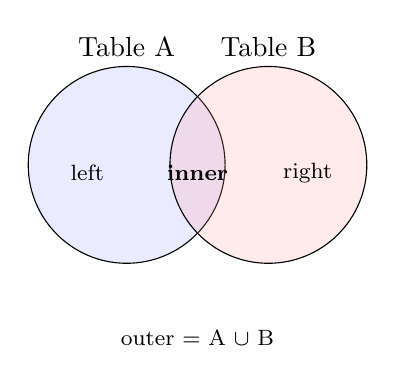
\begin{tikzpicture}[
  set/.style={circle, draw, minimum size=2.5cm, fill opacity=0.2, text opacity=1}
]
\node[set, fill=blue!40, label=above:{Table A}] (A) at (0,0) {};
\node[set, fill=red!40, label=above:{Table B}] (B) at (1.8,0) {};
\node at (0.9, -0.1) {\footnotesize\textbf{inner}};
\node at (-0.5, -0.1) {\footnotesize left};
\node at (2.3, -0.1) {\footnotesize right};
\node at (0.9, -2.2) {\footnotesize outer = A $\cup$ B};
\end{tikzpicture}
\end{center}

\section{Tri et classement}

\begin{codeblock}[title=\textbf{Python --- Tri}]
\begin{minted}{python}
# Trier par pourboire décroissant
top5 = tips.nlargest(5, 'tip')[['total_bill', 'tip', 'day']]
print(top5)

# Rang
tips['tip_rank'] = tips['tip'].rank(ascending=False).astype(int)
print(tips[['total_bill', 'tip', 'tip_rank']].head(5))
\end{minted}
\end{codeblock}

\begin{codeoutput}
\begin{verbatim}
     total_bill   tip  day
170       50.81 10.00  Sat
212       48.33  9.00  Sat
23        39.42  7.58  Sat
59        48.27  6.73  Sat
183       23.17  6.50  Sun

   total_bill   tip  tip_rank
0       16.99  1.01       224
1       10.34  1.66       188
2       21.01  3.50        52
3       23.68  3.31        63
4       24.59  3.61        46
\end{verbatim}
\end{codeoutput}

\section{Op\'erations sur les cha\^ines}

\begin{codeblock}[title=\textbf{Python --- Accesseur \texttt{.str}}]
\begin{minted}{python}
noms = pd.Series(['  Alice Dupont  ', 'bob martin', 'CHARLIE PETIT'])

print(noms.str.strip().str.title())
print(noms.str.contains('art', case=False))
\end{minted}
\end{codeblock}

\begin{codeoutput}
\begin{verbatim}
0     Alice Dupont
1       Bob Martin
2    Charlie Petit
dtype: object
0    False
1     True
2    False
dtype: bool
\end{verbatim}
\end{codeoutput}

\section{Exercices}

\begin{exercice}[$\star$]
Charger le jeu \py{tips} de Seaborn. Afficher le nombre de repas par jour de la semaine et par moment (d\'ejeuner/d\^iner).
\end{exercice}

\begin{exercice}[$\star$]
Cr\'eer un DataFrame avec 5 \'etudiants, leurs notes en maths et en physique. Ajouter une colonne <<~moyenne~>> et trier par moyenne d\'ecroissante.
\end{exercice}

\begin{exercice}[$\star\star$]
Sur le jeu Tips, calculer pour chaque combinaison (sexe, fumeur) : le nombre de repas, l'addition moyenne et le pourcentage moyen de pourboire.
\end{exercice}

\begin{exercice}[$\star\star$]
Cr\'eer deux DataFrames : un avec des produits (id, nom, cat\'egorie), un avec des ventes (id\_produit, quantit\'e, date). Les joindre et calculer le chiffre d'affaires par cat\'egorie.
\end{exercice}

\begin{exercice}[$\star\star\star$]
\'Ecrire une fonction qui prend un DataFrame et retourne un rapport automatique : nombre de lignes, types de colonnes, pourcentage de valeurs manquantes par colonne, nombre de doublons.
\end{exercice}

\begin{formules}[title=\textbf{Fonctions Pandas essentielles}]
\begin{itemize}
\item \py{pd.read_csv()}, \py{df.to_csv()} --- import/export
\item \py{df.head()}, \py{df.info()}, \py{df.describe()} --- exploration
\item \py{df.loc[]}, \py{df.iloc[]} --- s\'election
\item \py{df.groupby().agg()} --- agr\'egation
\item \py{pd.merge()} --- jointures
\item \py{df.sort_values()}, \py{df.nlargest()} --- tri
\end{itemize}
\end{formules}
